\section{The Great Journey} \label{TheGreatJourney}

The Great Journey is a side quest/event that can occur in multiple ways and/or for multiple purposes. This journey is modeled based on The Great Journey level from Halo 2 (as far as appearance).

\begin{center}
	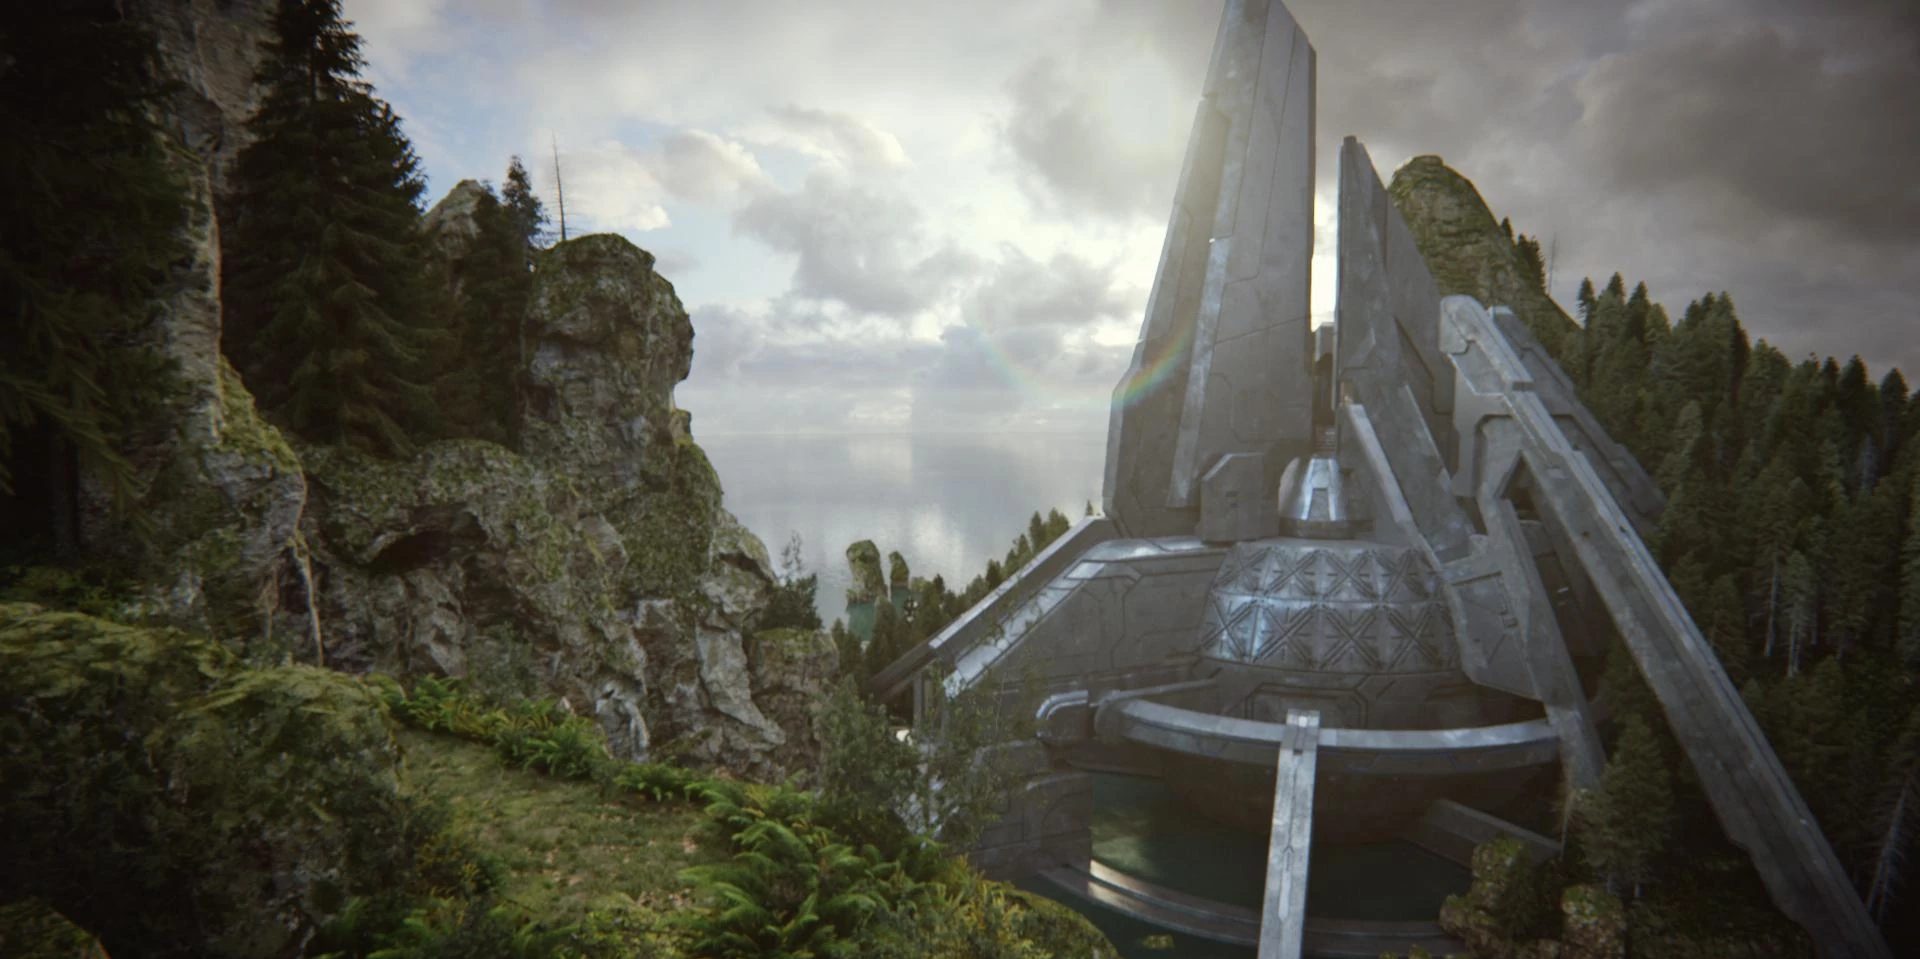
\includegraphics[width=\linewidth]{img/Halo/H2A_Mission_TheGreatJourney.jpg}
\end{center}

\subsubsection{The Eternal Neokoros Future Warning}

It can be an enhanced vision the players live through that is produced by the Eternal Neokoros. The visions purpose is to show the future that the Celestials will become if they are not stopped. The area features a research station that the Celestials are using to create advanced technologies for conquering areas that do not follow the Celestials. The party will encounter Celestial forces guarded with advanced shields and weaponry that make them incredibly hard to defeat. If they are found out as not being followers of the Celestials, they will be taken captive or executed on sight. They would also be heavily questioned as to how they came to be in this location which is hidden deep in a mountainous region. 

\subsubsection{Future events}

The region can also serve as an actual future event that the party gets teleported to. The area is in the Pluvian forest only in a future time. The area contains a large research station with advanced weaponry being created. The facility has armed workers on the outskirts near where the party members are located. The workers are not to tolerate intruders as the facility is top secret.

\subsubsection{Past events}

The region can serve as a past event. The party gets transported into the past. The facility they see can serve as a research base of Myrddin. This is the place where Merlin is discovering the abilities of magic and studying alternate dimensions. Only days earlier, they unlocked a rift to the void, unleashing a new set of physics on their physical world. Ever since, the area around Myrddin has been acting strange in the sense that things have been appearing and disappearing. The zone became unstable in space, time, and matter, which Myrddin later learns to harness to create the Trinity Stones. 

